\documentclass[xcolor=svgnames]{beamer}\usepackage[]{graphicx}\usepackage[]{color}
%% maxwidth is the original width if it is less than linewidth
%% otherwise use linewidth (to make sure the graphics do not exceed the margin)
\makeatletter
\def\maxwidth{ %
  \ifdim\Gin@nat@width>\linewidth
    \linewidth
  \else
    \Gin@nat@width
  \fi
}
\makeatother

\definecolor{fgcolor}{rgb}{0.345, 0.345, 0.345}
\newcommand{\hlnum}[1]{\textcolor[rgb]{0.686,0.059,0.569}{#1}}%
\newcommand{\hlstr}[1]{\textcolor[rgb]{0.192,0.494,0.8}{#1}}%
\newcommand{\hlcom}[1]{\textcolor[rgb]{0.678,0.584,0.686}{\textit{#1}}}%
\newcommand{\hlopt}[1]{\textcolor[rgb]{0,0,0}{#1}}%
\newcommand{\hlstd}[1]{\textcolor[rgb]{0.345,0.345,0.345}{#1}}%
\newcommand{\hlkwa}[1]{\textcolor[rgb]{0.161,0.373,0.58}{\textbf{#1}}}%
\newcommand{\hlkwb}[1]{\textcolor[rgb]{0.69,0.353,0.396}{#1}}%
\newcommand{\hlkwc}[1]{\textcolor[rgb]{0.333,0.667,0.333}{#1}}%
\newcommand{\hlkwd}[1]{\textcolor[rgb]{0.737,0.353,0.396}{\textbf{#1}}}%

\usepackage{framed}
\makeatletter
\newenvironment{kframe}{%
 \def\at@end@of@kframe{}%
 \ifinner\ifhmode%
  \def\at@end@of@kframe{\end{minipage}}%
  \begin{minipage}{\columnwidth}%
 \fi\fi%
 \def\FrameCommand##1{\hskip\@totalleftmargin \hskip-\fboxsep
 \colorbox{shadecolor}{##1}\hskip-\fboxsep
     % There is no \\@totalrightmargin, so:
     \hskip-\linewidth \hskip-\@totalleftmargin \hskip\columnwidth}%
 \MakeFramed {\advance\hsize-\width
   \@totalleftmargin\z@ \linewidth\hsize
   \@setminipage}}%
 {\par\unskip\endMakeFramed%
 \at@end@of@kframe}
\makeatother

\definecolor{shadecolor}{rgb}{.97, .97, .97}
\definecolor{messagecolor}{rgb}{0, 0, 0}
\definecolor{warningcolor}{rgb}{1, 0, 1}
\definecolor{errorcolor}{rgb}{1, 0, 0}
\newenvironment{knitrout}{}{} % an empty environment to be redefined in TeX

\usepackage{alltt}
\usetheme{Boadilla}
\usecolortheme[named=SeaGreen]{structure}
\usepackage{graphicx}
\usepackage{breqn}
\usepackage{xcolor}
\usepackage{booktabs}
\usepackage{verbatim}
\usepackage{tikz}
\usepackage{lmodern}
\usetikzlibrary{shadows,arrows,positioning}
\definecolor{links}{HTML}{2A1B81}
\hypersetup{colorlinks,linkcolor=links,urlcolor=links}
\usepackage{pgfpages}

\newcommand{\Bigtxt}[1]{\textbf{\textit{#1}}}
\IfFileExists{upquote.sty}{\usepackage{upquote}}{}
\begin{document}

\title[Exploratory Data Analysis]{Exploratory Data Analysis with SWMP}

\author[M. Beck, T. O'Brien]{Marcus W. Beck\inst{1} \and Todd D. O'Brien\inst{2}}

\date{}

\institute[]{\inst{1} ORISE, USEPA NHEERL Gulf Ecology Division\\ Email: \href{mailto:beck.marcus@epa.gov}{beck.marcus@epa.gov} \and \inst{2} NOAA/NMFS Copepod Project\\ Email: \href{todd.obrien@noaa.gov}{todd.obrien@noaa.gov}}

% knitr setup


% load SWMPr from local


%%%%%%
\begin{frame}
\vspace{0.3in}
\centerline{
\begin{tikzpicture}
  \node[drop shadow={shadow xshift=0ex,shadow yshift=0ex},fill=white,draw] at (0,0) {
\includegraphics[width=0.9\textwidth]{bg_main.jpg}};
\end{tikzpicture}}
\titlepage
\end{frame}

%%%%%%
\begin{frame}{Objectives and agenda}
\begin{itemize}
\onslide<+->
\item Objectives \\~\\
\begin{itemize}
\item What are some basic time series analysis techniques and when would you use them? \\~\\
\item How are the data set up, what functions are used, and how are the results interpreted? \\~\\
\end{itemize}
\onslide<+->
\item Agenda \\~\\
\begin{itemize}
\item Common functions for exploratory data analysis \\~\\
\item Analysis 1 - missing data and interpolation\\~\\
\item Analysis 2 - smoothing and aggregation \\~\\
\item Analysis 3 - basic trend analysis\\~\\
\end{itemize}
\end{itemize}
\end{frame}

%%%%%%
\begin{frame}{Interactive portion}
You can follow along in this module: \\~\\
\begin{itemize}
\item dataset3 \\~\\
\item script3 \\~\\
\end{itemize}
\Large
\centerline{\emph{Interactive!}}
\end{frame}

%%%%%%
\begin{frame}{Common functions for EDA}
What is exploratory data analysis (EDA)? \\~\\
A general term that describes preliminary evaluation of a variable or multiple variables in a dataset to assess quantitative properties for further analysis\\~\\
EDA can inform you of the \alert{types} of variables (categorical, continuous), \alert{distribution} of a variable (central tendency, spread), \alert{correlations} between variables, and presence of \alert{outliers} \\~\\
You may decide to omit variables or specific observations, transform, standardize, etc.\\~\\
Many of the same principles that apply to standard data analysis apply to time series analysis
\end{frame}

%%%%%%
\begin{frame}[containsverbatim]{Common functions for EDA}
R has many functions available for EDA - see the \href{http://cran.r-project.org/doc/contrib/Short-refcard.pdf}{R reference card} for some ideas\\~\\
We will cover a few basic techniques but keep in mind EDA is a general term and much of what we have already covered, and will cover, can be considered exploratory \\~\\
Let's import some data:

\begin{knitrout}\scriptsize
\definecolor{shadecolor}{rgb}{0.969, 0.969, 0.969}\color{fgcolor}\begin{kframe}
\begin{alltt}
\hlcom{# reload the SWMPr package if you started a new session}
\hlkwd{library}\hlstd{(SWMPr)}

\hlcom{# import data, qaqc, and subset}
\hlcom{# change this path for the flash drive}
\hlstd{path} \hlkwb{<-} \hlstr{'C:/data/dataset3'}
\hlstd{nut_dat} \hlkwb{<-} \hlkwd{import_local}\hlstd{(path,} \hlstr{'cbmmcnut'}\hlstd{)}
\hlstd{nut_dat} \hlkwb{<-} \hlkwd{qaqc}\hlstd{(nut_dat)}
\hlstd{nut_dat} \hlkwb{<-} \hlkwd{subset}\hlstd{(nut_dat,} \hlkwc{select} \hlstd{=} \hlkwd{c}\hlstd{(}\hlstr{'po4f'}\hlstd{,} \hlstr{'nh4f'}\hlstd{))}
\end{alltt}
\end{kframe}
\end{knitrout}
\end{frame}

%%%%%%
\begin{frame}[containsverbatim]{Common functions for EDA}
Perhaps the most useful function in R is `summary'
\begin{knitrout}\scriptsize
\definecolor{shadecolor}{rgb}{0.969, 0.969, 0.969}\color{fgcolor}\begin{kframe}
\begin{alltt}
\hlcom{# get a summary of the data}
\hlkwd{summary}\hlstd{(nut_dat)}
\end{alltt}
\begin{verbatim}
##  datetimestamp                      po4f          no23f       chla_n  
##  Min.   :2011-03-23 11:45:00   Min.   :0.00   Min.   :0   Min.   : 2  
##  1st Qu.:2011-09-15 22:37:30   1st Qu.:0.01   1st Qu.:0   1st Qu.: 5  
##  Median :2012-06-22 10:30:30   Median :0.02   Median :0   Median : 8  
##  Mean   :2012-07-13 12:56:29   Mean   :0.02   Mean   :0   Mean   :17  
##  3rd Qu.:2013-06-02 21:26:30   3rd Qu.:0.02   3rd Qu.:0   3rd Qu.:17  
##  Max.   :2013-12-04 11:46:00   Max.   :0.05   Max.   :0   Max.   :98  
##                                               NA's   :5   NA's   :4
\end{verbatim}
\end{kframe}
\end{knitrout}
\end{frame}

%%%%%%
\begin{frame}[containsverbatim]{Common functions for EDA}
The pairs function is useful for evaluating simple bivariate correlations
\begin{knitrout}\scriptsize
\definecolor{shadecolor}{rgb}{0.969, 0.969, 0.969}\color{fgcolor}\begin{kframe}
\begin{alltt}
\hlcom{# bivariate scatterplots}
\hlkwd{pairs}\hlstd{(nut_dat)}
\end{alltt}
\end{kframe}

{\centering 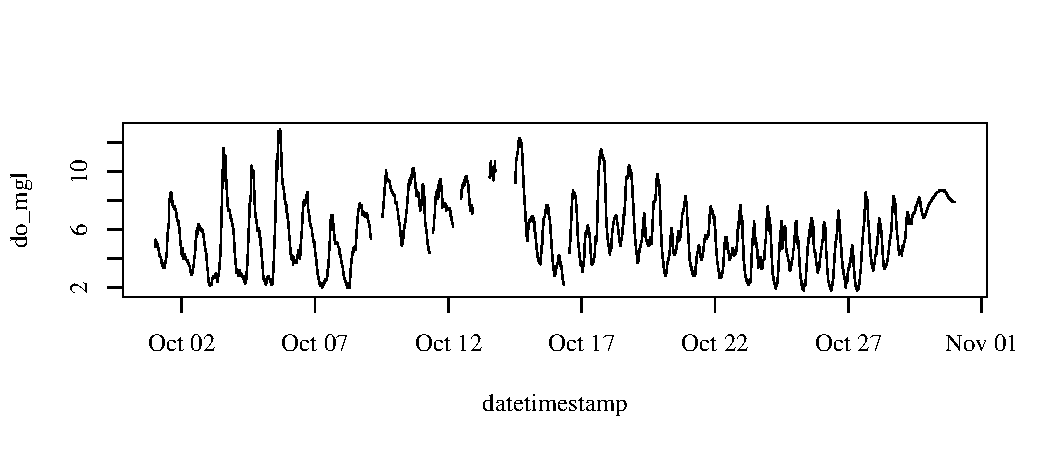
\includegraphics[width=0.5\textwidth]{figure/unnamed-chunk-4} 

}



\end{knitrout}
\end{frame}

%%%%%%
\begin{frame}[containsverbatim]{Common functions for EDA}
Histograms are useful...
\begin{knitrout}\scriptsize
\definecolor{shadecolor}{rgb}{0.969, 0.969, 0.969}\color{fgcolor}\begin{kframe}
\begin{alltt}
\hlcom{# some histograms}
\hlkwd{hist}\hlstd{(nut_dat}\hlopt{$}\hlstd{po4f)}
\hlkwd{hist}\hlstd{(nut_dat}\hlopt{$}\hlstd{no23f)}
\end{alltt}
\end{kframe}

{\centering 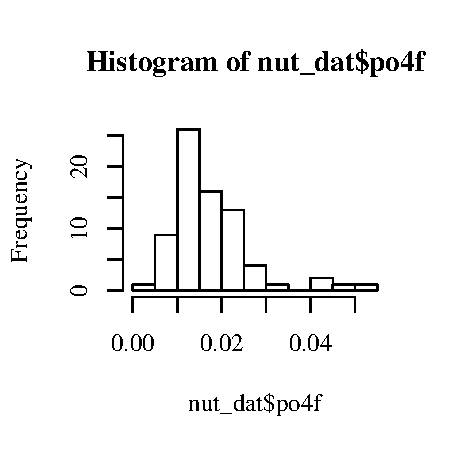
\includegraphics[width=0.4\textwidth]{figure/unnamed-chunk-51} 
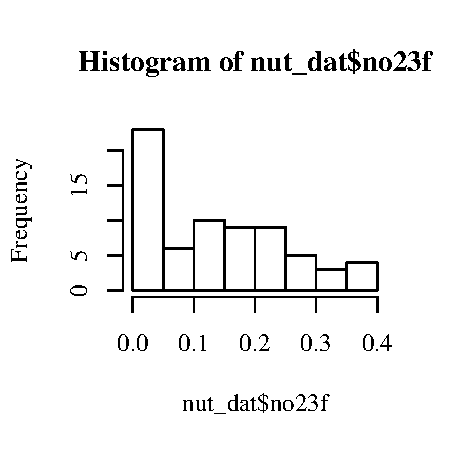
\includegraphics[width=0.4\textwidth]{figure/unnamed-chunk-52} 

}



\end{knitrout}
\end{frame}

%%%%%%
\begin{frame}[containsverbatim]{Common functions for EDA}
Boxplots are useful...
\begin{knitrout}\scriptsize
\definecolor{shadecolor}{rgb}{0.969, 0.969, 0.969}\color{fgcolor}\begin{kframe}
\begin{alltt}
\hlcom{# some boxplots}
\hlkwd{boxplot}\hlstd{(nut_dat}\hlopt{$}\hlstd{po4f,} \hlkwc{main} \hlstd{=} \hlstr{'p04f'}\hlstd{)}
\hlkwd{boxplot}\hlstd{(nut_dat}\hlopt{$}\hlstd{no23f,} \hlkwc{main} \hlstd{=} \hlstr{'no23f'}\hlstd{)}
\end{alltt}
\end{kframe}

{\centering 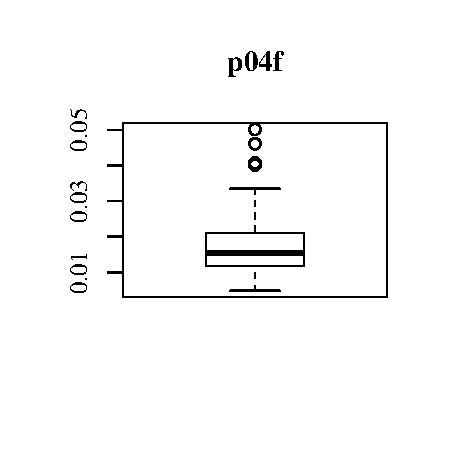
\includegraphics[width=0.4\textwidth]{figure/unnamed-chunk-61} 
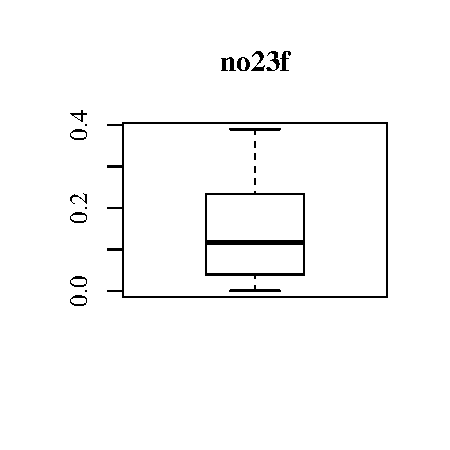
\includegraphics[width=0.4\textwidth]{figure/unnamed-chunk-62} 

}



\end{knitrout}
\end{frame}

%%%%%%
\begin{frame}{Common functions for EDA}
Plotting individual variables or simple scatterplots between two variables will get you familiar with a dataset\\~\\
Again, R has many functions for EDA and we don't want to focus on general approaches that can be learned at home \\~\\
A quick google search of `exploratory data analysis in r' will point you in the right direction \\~\\
For now, we will focus on some tasks that have specific relevance to SWMP
\end{frame}

%%%%%%
\begin{frame}[containsverbatim]{Analysis 1 - Missing data and interpolation}
Time series will usually include missing data - you will have to decide how to handle missing values \\~\\
Let's import some wq data

\begin{knitrout}\scriptsize
\definecolor{shadecolor}{rgb}{0.969, 0.969, 0.969}\color{fgcolor}\begin{kframe}
\begin{alltt}
\hlcom{# import data, qaqc, and subset}
\hlcom{# change this path for the flash drive}
\hlstd{path} \hlkwb{<-} \hlstr{'C:/data/dataset3'}
\hlstd{wq_dat} \hlkwb{<-} \hlkwd{import_local}\hlstd{(path,} \hlstr{'cbmmcwq2012'}\hlstd{)}
\end{alltt}
\end{kframe}
\end{knitrout}
\begin{knitrout}\scriptsize
\definecolor{shadecolor}{rgb}{0.969, 0.969, 0.969}\color{fgcolor}\begin{kframe}
\begin{alltt}
\hlcom{# remove qaqc, and subset do_mgl}
\hlstd{wq_dat} \hlkwb{<-} \hlkwd{qaqc}\hlstd{(wq_dat)}
\hlstd{wq_dat} \hlkwb{<-} \hlkwd{subset}\hlstd{(wq_dat,} \hlkwc{select} \hlstd{=} \hlstr{'do_mgl'}\hlstd{)}

\hlcom{# how many missing values?}
\hlkwd{sum}\hlstd{(}\hlkwd{is.na}\hlstd{(wq_dat}\hlopt{$}\hlstd{do_mgl))}
\end{alltt}
\begin{verbatim}
## [1] 419
\end{verbatim}
\end{kframe}
\end{knitrout}
\end{frame}

%%%%%%
\begin{frame}[containsverbatim]{Analysis 1 - Missing data and interpolation}
Mising data can be removed with the subset function or replaced with the mean
\begin{knitrout}\scriptsize
\definecolor{shadecolor}{rgb}{0.969, 0.969, 0.969}\color{fgcolor}\begin{kframe}
\begin{alltt}
\hlcom{# a temporary object so we don't overwrite wq_dat}
\hlstd{wq_tmp} \hlkwb{<-} \hlstd{wq_dat}

\hlcom{# remove missing values with subset function}
\hlstd{wq_tmp} \hlkwb{<-} \hlkwd{subset}\hlstd{(wq_tmp,} \hlkwc{rem_row} \hlstd{= T)}

\hlcom{# or replace missing values with the mean}
\hlstd{wq_tmp} \hlkwb{<-} \hlstd{wq_dat}
\hlstd{wq_tmp[}\hlkwd{is.na}\hlstd{(wq_tmp}\hlopt{$}\hlstd{do_mgl),} \hlstr{'do_mgl'}\hlstd{]} \hlkwb{<-} \hlkwd{mean}\hlstd{(wq_tmp}\hlopt{$}\hlstd{do_mgl,} \hlkwc{na.rm} \hlstd{= T)}
\end{alltt}
\end{kframe}
\end{knitrout}
What are some issues with these approaches? \\~\\
`subset' will change the time step \\~\\
Neither approach is very true to the data... 
\end{frame}

%%%%%%
\begin{frame}[containsverbatim]{Analysis 1 - Missing data and interpolation}
Introducing the `na.approx' function - this method can interpolate missing data
\begin{knitrout}\scriptsize
\definecolor{shadecolor}{rgb}{0.969, 0.969, 0.969}\color{fgcolor}\begin{kframe}
\begin{alltt}
\hlcom{# subset the do time series for plotting}
\hlstd{wq_dat} \hlkwb{<-} \hlkwd{subset}\hlstd{(wq_dat,} \hlkwc{subset} \hlstd{=} \hlkwd{c}\hlstd{(}\hlstr{'2012-10-01 0:0'}\hlstd{,} \hlstr{'2012-10-31 0:0'}\hlstd{))}
\hlkwd{plot}\hlstd{(do_mgl} \hlopt{~} \hlstd{datetimestamp, wq_dat,} \hlkwc{type} \hlstd{=} \hlstr{'l'}\hlstd{)}
\end{alltt}
\end{kframe}

{\centering 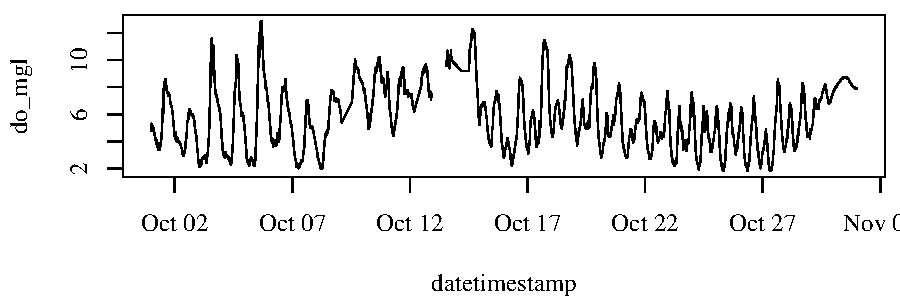
\includegraphics[width=0.8\textwidth]{figure/unnamed-chunk-11} 

}



\end{knitrout}
Notice the missing values around October 12\textsuperscript{th}
\end{frame}

%%%%%%
\begin{frame}[containsverbatim]{Analysis 1 - Missing data and interpolation}
Here's what the time series looks like after using `na.approx'
\begin{knitrout}\scriptsize
\definecolor{shadecolor}{rgb}{0.969, 0.969, 0.969}\color{fgcolor}

{\centering 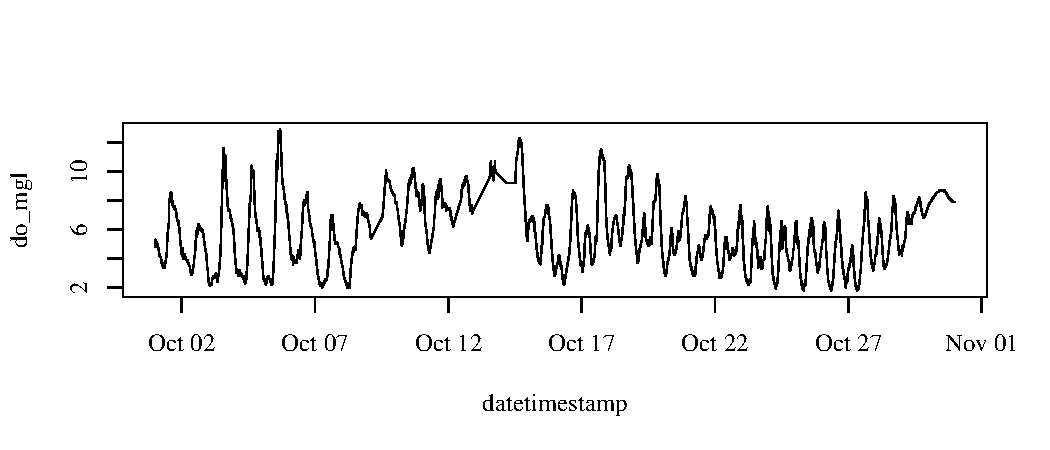
\includegraphics[width=0.8\textwidth]{figure/unnamed-chunk-12} 

}



\end{knitrout}
The missing values have been linearly interpolated - not a true representation but better than some other approaches
\end{frame}

%%%%%%
\begin{frame}[containsverbatim]{Analysis 1 - Missing data and interpolation}
The `na.approx' function has only a few arguments
\end{frame}

%%%%%%
\begin{frame}
\vspace{0.3in}
\centerline{
\begin{tikzpicture}
  \node[drop shadow={shadow xshift=0ex,shadow yshift=0ex},fill=white,draw] at (0,0) {
\includegraphics[width=0.9\textwidth]{bg_main.jpg}};
\end{tikzpicture}}
\vspace{0.5in}
\Large
\centerline{\Bigtxt{Questions??}}
\end{frame}

\end{document}
